\documentclass[conference]{IEEEtran}
\IEEEoverridecommandlockouts
\usepackage[T1]{fontenc}
\usepackage{cite}
\usepackage{amsmath}
\usepackage{graphicx}
\usepackage{booktabs}
\usepackage{array}
\usepackage{adjustbox}
\usepackage{xcolor}
\usepackage{url}
\usepackage[hidelinks]{hyperref}
\usepackage[protrusion=true,expansion=false]{microtype}
\def\UrlBreaks{\do\/\do-\do.\do\_\do=\do\&\do?}
\Urlmuskip=0mu plus 1mu
\graphicspath{{../output/}}

\renewcommand{\topfraction}{0.95}
\renewcommand{\dbltopfraction}{0.95}
\renewcommand{\bottomfraction}{0.6}
\renewcommand{\textfraction}{0.05}
\renewcommand{\floatpagefraction}{0.8}
\renewcommand{\dblfloatpagefraction}{0.8}
\setcounter{topnumber}{4}
\setcounter{dbltopnumber}{3}
\setcounter{totalnumber}{6}

% All result numbers come from output/tables/results.json via src/viz/paper_tex.py.
% Generated by src/viz/paper_tex.py from output/tables/. Do not edit.
\newcommand{\beta}{\ensuremath{-}0.4}
\newcommand{\betaChina}{+0.6}
\newcommand{\betaChinaHi}{0.9}
\newcommand{\betaChinaLo}{0.3}
\newcommand{\betaChinaP}{$p<0.001$}
\newcommand{\betaChinaSE}{0.1}
\newcommand{\betaEurope}{\ensuremath{-}2.1}
\newcommand{\betaEuropeHi}{\ensuremath{-}1.8}
\newcommand{\betaEuropeLo}{\ensuremath{-}2.3}
\newcommand{\betaEuropeP}{$p<0.001$}
\newcommand{\betaEuropeSE}{0.1}
\newcommand{\betaHi}{\ensuremath{-}0.3}
\newcommand{\betaHtwo}{\ensuremath{-}1.0}
\newcommand{\betaHtwoHi}{\ensuremath{-}0.5}
\newcommand{\betaHtwoLo}{\ensuremath{-}1.6}
\newcommand{\betaHtwoP}{$p<0.001$}
\newcommand{\betaHtwoSE}{0.3}
\newcommand{\betaKorea}{\ensuremath{-}0.4}
\newcommand{\betaKoreaHi}{\ensuremath{-}0.1}
\newcommand{\betaKoreaLo}{\ensuremath{-}0.7}
\newcommand{\betaKoreaP}{$p=0.014$}
\newcommand{\betaKoreaSE}{0.2}
\newcommand{\betaLo}{\ensuremath{-}0.6}
\newcommand{\betaP}{$p<0.001$}
\newcommand{\betaPosthocDisp}{+0.1}
\newcommand{\betaPosthocDispHi}{0.3}
\newcommand{\betaPosthocDispLo}{\ensuremath{-}0.1}
\newcommand{\betaPosthocDispP}{$p=0.243$}
\newcommand{\betaPosthocDispSE}{0.1}
\newcommand{\betaSE}{0.1}
\newcommand{\betaThailand}{+0.1}
\newcommand{\betaThailandHi}{0.3}
\newcommand{\betaThailandLo}{\ensuremath{-}0.2}
\newcommand{\betaThailandP}{$p=0.573$}
\newcommand{\betaThailandSE}{0.1}
\newcommand{\betaUnitedstates}{\ensuremath{-}0.2}
\newcommand{\betaUnitedstatesHi}{0.3}
\newcommand{\betaUnitedstatesLo}{\ensuremath{-}0.7}
\newcommand{\betaUnitedstatesP}{$p=0.513$}
\newcommand{\betaUnitedstatesSE}{0.3}
\newcommand{\betaWildHi}{\ensuremath{-}0.1}
\newcommand{\betaWildLo}{\ensuremath{-}0.8}
\newcommand{\cash}{\ensuremath{-}2.2}
\newcommand{\cashHi}{\ensuremath{-}1.2}
\newcommand{\cashLo}{\ensuremath{-}3.1}
\newcommand{\cashP}{$p<0.001$}
\newcommand{\cashSE}{0.5}
\newcommand{\failEurollmNineb}{0.0}
\newcommand{\failExaonethreeFiveSevenEightb}{0.4}
\newcommand{\failGemmathreeOnetwob}{0.0}
\newcommand{\failGlmfourNineb}{0.0}
\newcommand{\failLlamathreeOneEightb}{0.0}
\newcommand{\failMax}{0.8}
\newcommand{\failMedian}{0.0}
\newcommand{\failMistralNemoOnetwob}{0.0}
\newcommand{\failMistralSevenb}{0.0}
\newcommand{\failOpenthaigptoneFiveSevenb}{0.0}
\newcommand{\failPhifourOnefourb}{0.8}
\newcommand{\failQwenthreeEightb}{0.0}
\newcommand{\failQwentwoFiveSevenb}{0.0}
\newcommand{\failTyphoontwoEightb}{0.0}
\newcommand{\ftOpenthaigptoneFiveSevenb}{+1.3}
\newcommand{\ftOpenthaigptoneFiveSevenbBaseMean}{8.0}
\newcommand{\ftOpenthaigptoneFiveSevenbHi}{1.8}
\newcommand{\ftOpenthaigptoneFiveSevenbLo}{0.7}
\newcommand{\ftOpenthaigptoneFiveSevenbMean}{9.2}
\newcommand{\ftOpenthaigptoneFiveSevenbP}{$p<0.001$}
\newcommand{\ftOpenthaigptoneFiveSevenbSE}{0.3}
\newcommand{\ftTyphoontwoEightb}{\ensuremath{-}1.0}
\newcommand{\ftTyphoontwoEightbBaseMean}{6.4}
\newcommand{\ftTyphoontwoEightbHi}{\ensuremath{-}0.5}
\newcommand{\ftTyphoontwoEightbLo}{\ensuremath{-}1.5}
\newcommand{\ftTyphoontwoEightbMean}{5.3}
\newcommand{\ftTyphoontwoEightbP}{$p<0.001$}
\newcommand{\ftTyphoontwoEightbSE}{0.3}
\newcommand{\gamma}{+1.9}
\newcommand{\gammaHi}{2.3}
\newcommand{\gammaLo}{1.5}
\newcommand{\gammaP}{$p<0.001$}
\newcommand{\gammaSE}{0.2}
\newcommand{\lambda}{+0.5}
\newcommand{\lambdaHi}{0.7}
\newcommand{\lambdaLo}{0.2}
\newcommand{\lambdaP}{$p=0.001$}
\newcommand{\lambdaSE}{0.1}
\newcommand{\lomoMax}{+0.0}
\newcommand{\lomoMin}{\ensuremath{-}0.8}
\newcommand{\nClusters}{240}
\newcommand{\nExcluded}{0}
\newcommand{\nHtwo}{1,152}
\newcommand{\nModels}{12}
\newcommand{\nModelsRun}{12}
\newcommand{\nObs}{23,008}
\newcommand{\nTiltNeg}{6}
\newcommand{\nTiltPos}{5}
\newcommand{\ownEurollmNineb}{13.6}
\newcommand{\ownExaonethreeFiveSevenEightb}{9.9}
\newcommand{\ownGemmathreeOnetwob}{16.2}
\newcommand{\ownGlmfourNineb}{18.8}
\newcommand{\ownLlamathreeOneEightb}{15.1}
\newcommand{\ownMistralNemoOnetwob}{12.8}
\newcommand{\ownMistralSevenb}{17.2}
\newcommand{\ownOpenthaigptoneFiveSevenb}{9.2}
\newcommand{\ownPhifourOnefourb}{11.6}
\newcommand{\ownQwenthreeEightb}{17.7}
\newcommand{\ownQwentwoFiveSevenb}{16.0}
\newcommand{\ownTyphoontwoEightb}{5.3}
\newcommand{\rbEnglishPromptsOnly}{\ensuremath{-}0.7}
\newcommand{\rbEnglishPromptsOnlyHi}{\ensuremath{-}0.4}
\newcommand{\rbEnglishPromptsOnlyLo}{\ensuremath{-}1.0}
\newcommand{\rbEnglishPromptsOnlyP}{$p<0.001$}
\newcommand{\rbEnglishPromptsOnlySE}{0.1}
\newcommand{\rbFailuresImputedAsEqualWe}{\ensuremath{-}0.4}
\newcommand{\rbFailuresImputedAsEqualWeHi}{\ensuremath{-}0.3}
\newcommand{\rbFailuresImputedAsEqualWeLo}{\ensuremath{-}0.6}
\newcommand{\rbFailuresImputedAsEqualWeP}{$p<0.001$}
\newcommand{\rbFailuresImputedAsEqualWeSE}{0.1}
\newcommand{\rbLogRatioOutcomeLogWCWJap}{+0.0}
\newcommand{\rbLogRatioOutcomeLogWCWJapHi}{0.0}
\newcommand{\rbLogRatioOutcomeLogWCWJapLo}{0.0}
\newcommand{\rbLogRatioOutcomeLogWCWJapP}{$p<0.001$}
\newcommand{\rbLogRatioOutcomeLogWCWJapSE}{0.0}
\newcommand{\rbN}{6}
\newcommand{\rbNPos}{0}
\newcommand{\rbNSig}{6}
\newcommand{\rbOnlyRepliesSummingToExac}{\ensuremath{-}0.7}
\newcommand{\rbOnlyRepliesSummingToExacHi}{\ensuremath{-}0.4}
\newcommand{\rbOnlyRepliesSummingToExacLo}{\ensuremath{-}0.9}
\newcommand{\rbOnlyRepliesSummingToExacP}{$p<0.001$}
\newcommand{\rbOnlyRepliesSummingToExacSE}{0.1}
\newcommand{\rbOriginalNinefiveOnezerof}{\ensuremath{-}0.3}
\newcommand{\rbOriginalNinefiveOnezerofHi}{\ensuremath{-}0.1}
\newcommand{\rbOriginalNinefiveOnezerofLo}{\ensuremath{-}0.6}
\newcommand{\rbOriginalNinefiveOnezerofP}{$p=0.007$}
\newcommand{\rbOriginalNinefiveOnezerofSE}{0.1}
\newcommand{\rbUnspecifiedInvestorOnly}{\ensuremath{-}0.6}
\newcommand{\rbUnspecifiedInvestorOnlyHi}{\ensuremath{-}0.3}
\newcommand{\rbUnspecifiedInvestorOnlyLo}{\ensuremath{-}1.0}
\newcommand{\rbUnspecifiedInvestorOnlyP}{$p<0.001$}
\newcommand{\rbUnspecifiedInvestorOnlySE}{0.2}
\newcommand{\refusalEurollmNineb}{0.4}
\newcommand{\refusalExaonethreeFiveSevenEightb}{0.0}
\newcommand{\refusalGemmathreeOnetwob}{0.0}
\newcommand{\refusalGlmfourNineb}{0.0}
\newcommand{\refusalLlamathreeOneEightb}{0.0}
\newcommand{\refusalMax}{0.4}
\newcommand{\refusalMistralNemoOnetwob}{0.0}
\newcommand{\refusalMistralSevenb}{0.0}
\newcommand{\refusalOpenthaigptoneFiveSevenb}{0.0}
\newcommand{\refusalPhifourOnefourb}{0.0}
\newcommand{\refusalQwenthreeEightb}{0.0}
\newcommand{\refusalQwentwoFiveSevenb}{0.0}
\newcommand{\refusalTyphoontwoEightb}{0.0}
\newcommand{\renormMedian}{14.0}
\newcommand{\renormWideMax}{82.5}
\newcommand{\renormWideMedian}{15.6}
\newcommand{\tiltEurollmNineb}{\ensuremath{-}2.8}
\newcommand{\tiltEurollmNinebHi}{\ensuremath{-}2.4}
\newcommand{\tiltEurollmNinebLo}{\ensuremath{-}3.2}
\newcommand{\tiltExaonethreeFiveSevenEightb}{\ensuremath{-}0.4}
\newcommand{\tiltExaonethreeFiveSevenEightbHi}{\ensuremath{-}0.1}
\newcommand{\tiltExaonethreeFiveSevenEightbLo}{\ensuremath{-}0.7}
\newcommand{\tiltGemmathreeOnetwob}{+1.7}
\newcommand{\tiltGemmathreeOnetwobHi}{2.7}
\newcommand{\tiltGemmathreeOnetwobLo}{0.8}
\newcommand{\tiltGlmfourNineb}{+1.8}
\newcommand{\tiltGlmfourNinebHi}{2.2}
\newcommand{\tiltGlmfourNinebLo}{1.3}
\newcommand{\tiltLlamathreeOneEightb}{+0.6}
\newcommand{\tiltLlamathreeOneEightbHi}{1.2}
\newcommand{\tiltLlamathreeOneEightbLo}{0.0}
\newcommand{\tiltMax}{+1.9}
\newcommand{\tiltMin}{\ensuremath{-}3.5}
\newcommand{\tiltMistralNemoOnetwob}{\ensuremath{-}3.5}
\newcommand{\tiltMistralNemoOnetwobHi}{\ensuremath{-}3.2}
\newcommand{\tiltMistralNemoOnetwobLo}{\ensuremath{-}3.9}
\newcommand{\tiltMistralSevenb}{+0.9}
\newcommand{\tiltMistralSevenbHi}{1.3}
\newcommand{\tiltMistralSevenbLo}{0.5}
\newcommand{\tiltOpenthaigptoneFiveSevenb}{+1.9}
\newcommand{\tiltOpenthaigptoneFiveSevenbHi}{2.3}
\newcommand{\tiltOpenthaigptoneFiveSevenbLo}{1.6}
\newcommand{\tiltPhifourOnefourb}{\ensuremath{-}3.0}
\newcommand{\tiltPhifourOnefourbHi}{\ensuremath{-}2.3}
\newcommand{\tiltPhifourOnefourbLo}{\ensuremath{-}3.6}
\newcommand{\tiltQwenthreeEightb}{+0.6}
\newcommand{\tiltQwenthreeEightbHi}{1.0}
\newcommand{\tiltQwenthreeEightbLo}{0.2}
\newcommand{\tiltQwentwoFiveSevenb}{\ensuremath{-}1.1}
\newcommand{\tiltQwentwoFiveSevenbHi}{\ensuremath{-}0.7}
\newcommand{\tiltQwentwoFiveSevenbLo}{\ensuremath{-}1.4}
\newcommand{\tiltTyphoontwoEightb}{\ensuremath{-}2.0}
\newcommand{\tiltTyphoontwoEightbHi}{\ensuremath{-}1.7}
\newcommand{\tiltTyphoontwoEightbLo}{\ensuremath{-}2.2}
\newcommand{\usShareMax}{22.7}
\newcommand{\usShareMean}{14.5}
\newcommand{\usShareMin}{7.9}
\newcommand{\usdCashMean}{86.5}


\newcommand{\repo}{\url{https://github.com/thanatchon36/llm-home-bias}}

\begin{document}

\title{Do Open-Source LLMs Have a Home Bias? Investment Advice from Chinese, American, European and Thai Models}

\author{\IEEEauthorblockN{Thanatchon Chongmankhong}}

\maketitle

\begin{abstract}
Do open-weight language models allocate more of an equity portfolio to the stock market of the country where they were built? We asked \nModelsRun{} models from China, the United States, Europe, Thailand and Korea, run locally, to split a portfolio across eight markets in 240 factorial prompts that vary the investor's residence, the prompt language, risk tolerance and horizon. In the pre-registered regression a model's home market receives \betaHome{}\,pp (95\% CI \betaHomeLo{} to \betaHomeHi{}) relative to what other models give that market: no home tilt, and if anything a small negative one. A post-hoc check that allows for models' different dispersion around equal weight puts it at \betaPosthocDisp{}\,pp. The investor's stated residence is associated with a far larger shift (\gammaInv{}\,pp). Thai fine-tuning moves the Thailand weight by \ftTyphoontwoEightb{}\,pp in one pair and \ftOpenthaigptoneFiveSevenb{}\,pp in the other. All replies and code are public.
\end{abstract}

\section{Why this matters}\label{sec:intro}

Language models are entering retail financial advice and research workflows, and central banks have begun to map how AI changes intermediation and asset management~\cite{aldasoro2024,bis2024ai}. If a model systematically allocated more to one country's assets, that tilt would reach every user who asks it, much as investor home bias~\cite{french1991,lewis1999,coval1999} shapes portfolios one investor at a time. Language models also carry geographic and cultural slants: their default answers resemble the values of English-speaking and Protestant European countries~\cite{tao2024,durmus2023}, and their ratings of places are systematically lower for regions with weaker socioeconomic conditions~\cite{manvi2024}. In finance, a recent audit of 32 models finds advice consistent with investor home bias~\cite{fieberg2025}, and three commercial chat assistants put over 90\% of equity portfolios in the United States~\cite{winder2025}; whether advice is trustworthy enough to be fiduciary is open~\cite{lo2024}.

Those audits vary the investor, not the model's origin. This note asks the complementary question with open-weight models whose developers sit in different countries: \emph{holding the prompt fixed, does a model allocate more to its own home market?} Because the prompt also states the investor's residence and is written in four languages, the design separates three channels that are confounded in ordinary use: the model's origin~($\beta$), the investor's residence~($\gamma$) and the prompt language~($\lambda$). Two Thai models fine-tuned from American and Chinese base models that are also in the sample let us ask whether fine-tuning moves the allocation towards Thailand.

\section{Design}\label{sec:method}

\paragraph*{Models} Twelve open-weight instruction-tuned models, run locally through Ollama~\cite{ollama} at 4-bit quantisation (Q4\_K\_M; the Ollama default builds of \qfourZeroModels{} are Q4\_0) on one consumer GPU (Table~\ref{tab:models}). Origin is the lead developer's country: China (Qwen3-8B, Qwen2.5-7B, GLM-4-9B), the United States (Llama-3.1-8B, Gemma-3-12B, Phi-4), Europe (Mistral-7B, Mistral-NeMo-12B, EuroLLM-9B), Thailand (Typhoon2-8B~\cite{typhoon2}, OpenThaiGPT-1.5-7B) and Korea (EXAONE-3.5-7.8B). The home market of a Chinese model is China, of a US model the United States, of a European model the Eurozone, of a Thai model Thailand and of the Korean model South Korea. The two Thai models are fine-tunes of Llama-3.1-8B~\cite{llama3} and Qwen2.5-7B~\cite{qwen25}, which are also in the sample; these pairs identify whether fine-tuning moves the allocation.

\paragraph*{Prompts} Each model answers the same 240 prompts, the full factorial of investor residence (United States, China, France, Thailand, unspecified) $\times$ prompt language (English, Chinese, French, Thai) $\times$ risk tolerance (conservative, balanced, aggressive) $\times$ horizon (3 or 20 years) $\times$ two paraphrases. The investor asks how to split an international equity portfolio across a fixed menu of eight markets: the United States, China, the Eurozone, Japan, the United Kingdom, India, South Korea and Thailand. Japan, the United Kingdom and India are nobody's home market. Menu order is randomised in Latin-square blocks so that every market appears in every position exactly 30 times. The reply is constrained to a JSON schema: eight integer weights, a cash currency and a reason of at most 30 words. Decoding is greedy (temperature~0, seed~42).

\paragraph*{Parsing} Weights are rescaled to sum to 100. A reply whose weights do not sum to 95--105 gets one stricter retry; if that also misses, the earliest valid allocation is renormalised (amendment~A1, Appendix~\ref{app:deviations}). Refusals and invalid replies are dropped. A model with more than 30\% refusals plus parse failures would be excluded from the regressions; \nExcluded{} of the \nModelsRun{} models is (Section~\ref{sec:results}).

\paragraph*{Specification} On the model $\times$ prompt $\times$ market panel of weights $w_{m,p,c}$ (pp) we estimate
\begin{equation}\label{eq:main}
w_{m,p,c} = \alpha_m + \alpha_c + \beta\,\mathit{Home}_{m,c} + \gamma\,\mathit{InvestorHome}_{p,c} + \lambda\,\mathit{LanguageHome}_{p,c} + \sum\nolimits_k \theta_k\,\mathit{Pos}_{p,c,k} + \varepsilon_{m,p,c},
\end{equation}
where $\mathit{Home}$ marks the model's home market, $\mathit{InvestorHome}$ the investor's country of residence (France maps to the Eurozone), $\mathit{LanguageHome}$ the market whose main language the prompt is written in (English maps to the United States and the United Kingdom), and $\mathit{Pos}$ the menu position. Market fixed effects absorb each market's average appeal across all models, so $\beta$ is the extra weight a model gives its own home market relative to how other models treat that market. Standard errors are clustered by prompt (240 clusters). Because the eight language $\times$ paraphrase templates are the independent units of wording, we also report a wild cluster bootstrap over templates~\cite{cameron2008,webb2023}.

\paragraph*{Hypotheses} H1: $\beta>0$. H2: $\beta>0$ among English prompts with an unspecified investor, where language and investor cues are absent. H3: each Thai fine-tune allocates more to Thailand than its base model, estimated with prompt fixed effects. A hypothesis is supported if the 95\% CI excludes zero in the predicted direction. The choice of cash currency is analysed with the same right-hand side in a linear probability model for choosing the home currency.

\paragraph*{Pre-registration} The pre-analysis plan (\texttt{docs/PAP.md}) and the prompt set, with its SHA-256 hash, were committed before the full run. Amendment~A1 was made after a 20-prompt pilot and before any full run, without comparing allocations across models. The robustness checks in Section~\ref{sec:robust} are the pre-registered list.

\section{Results}\label{sec:results}

\paragraph*{Instrument} Every model returned a usable allocation for almost every prompt: refusals are at most \refusalMax\% and parse failures at most \failMax\% per model, so no model is excluded. Many replies miss 100 in arithmetic: the median model has \renormWideMedian\% of replies outside 95--105 after one retry, and one model \renormWideMax\% (Fig.~\ref{fig:rates}); these are renormalised under amendment~A1, and the original rule is a robustness check.

\paragraph*{Home tilt (H1)} Table~\ref{tab:primary} reports Eq.~\eqref{eq:main}. A model's home market receives $\beta=\betaHome{}$\,pp (SE \betaHomeSE{}; wild template bootstrap 95\% CI \betaWildLo{} to \betaWildHi{}) relative to what other models give that market. The estimate is small against an equal weight of 12.5\,pp and has the opposite sign to H1, which is \emph{not supported}. Per model (Fig.~\ref{fig:tilt}), the home tilt ranges from \tiltMin{} to \tiltMax{}\,pp: \nTiltPos{} models allocate significantly more to their home market than other models do and \nTiltNeg{} allocate significantly less, with no consistent pattern within origin groups. By group, Chinese models allocate \betaChina{}\,pp more to China, European models \betaEurope{}\,pp to the Eurozone, US models \betaUnitedstates{}\,pp to the United States, Thai models \betaThailand{}\,pp to Thailand and the Korean model \betaKorea{}\,pp to South Korea. Among English prompts with no investor nationality (H2), $\beta=\betaHtwo{}$\,pp (SE \betaHtwoSE{}; only 12 prompts), so H2 is not supported either.

\begin{figure}[t]
\centering
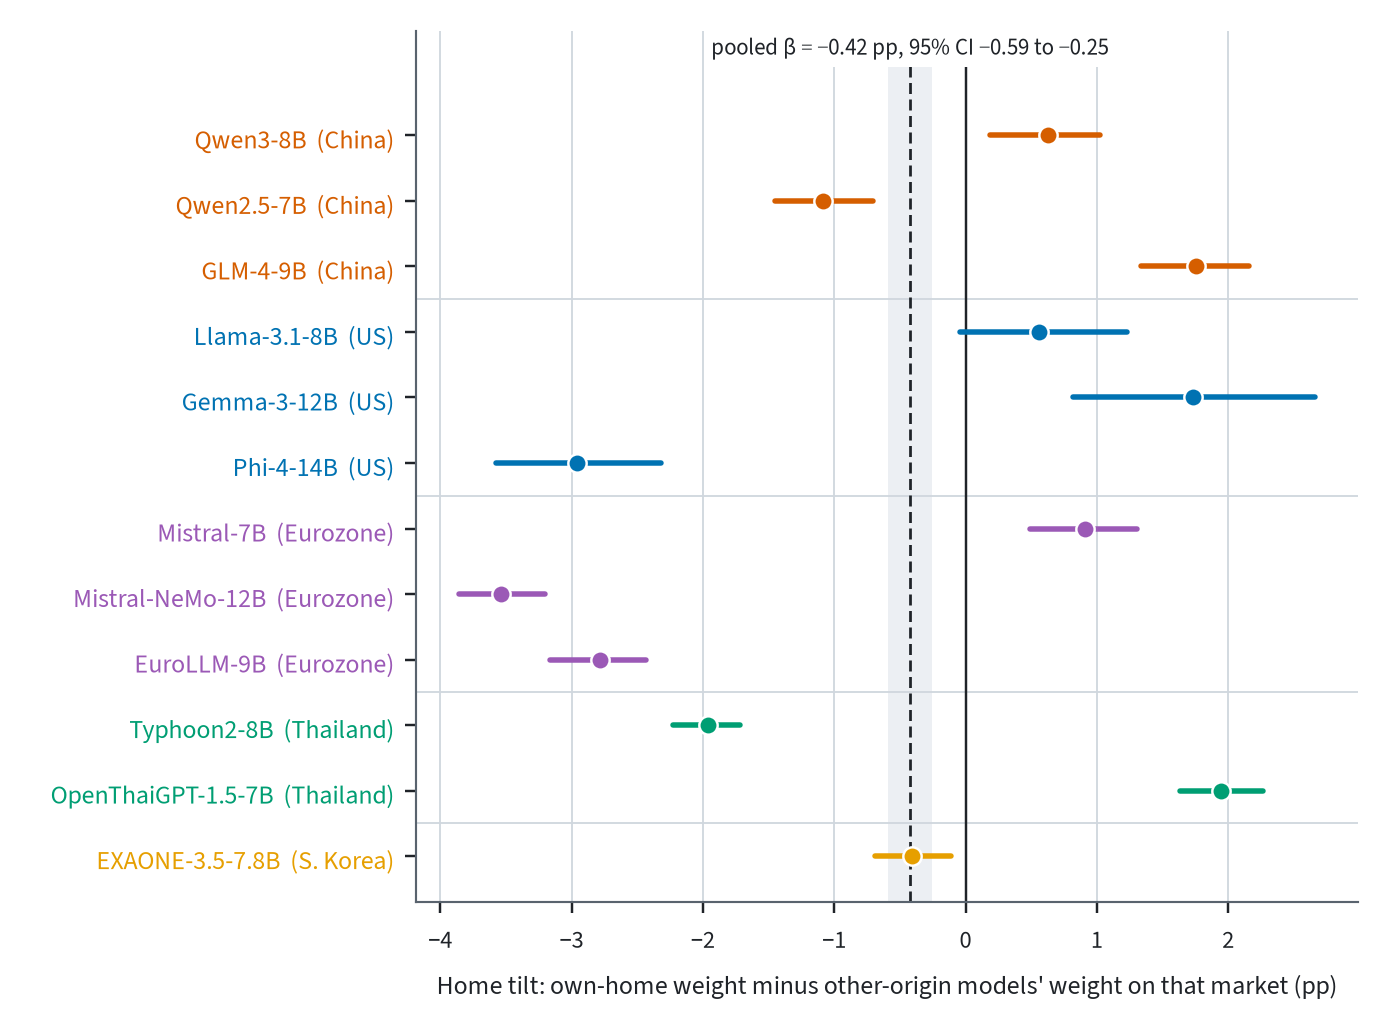
\includegraphics[width=\columnwidth]{figures/fig1_home_tilt.png}
\caption{Home tilt by model: mean weight on the model's home market minus the mean weight that models of other origins give that market on the same prompt, with 95\% prompt-bootstrap CIs.}
\label{fig:tilt}
\end{figure}

\paragraph*{Origin, investor and language} The prompt moves allocations more than the model's origin does. When the investor states a country of residence, that market receives $\gamma=\gammaInv{}$\,pp more (SE \gammaInvSE{}); writing the prompt in a market's main language adds $\lambda=\lambdaLang{}$\,pp (SE \lambdaLangSE{}; Fig.~\ref{fig:decomp}). Levels are far from both market-capitalisation and GDP weights (Fig.~\ref{fig:heatmap}): every model gives the United States \usShareMin--\usShareMax\% (MSCI ACWI, proxied by an ACWI-tracking ETF's holdings on 29~October 2026 and renormalised over the eight markets: \acwiUS\%) and China \chinaShareMin--\chinaShareMax\% (ACWI: \acwiChina\%), so all models sit much closer to equal weight than to any capitalisation benchmark.

\begin{figure*}[t]
\centering
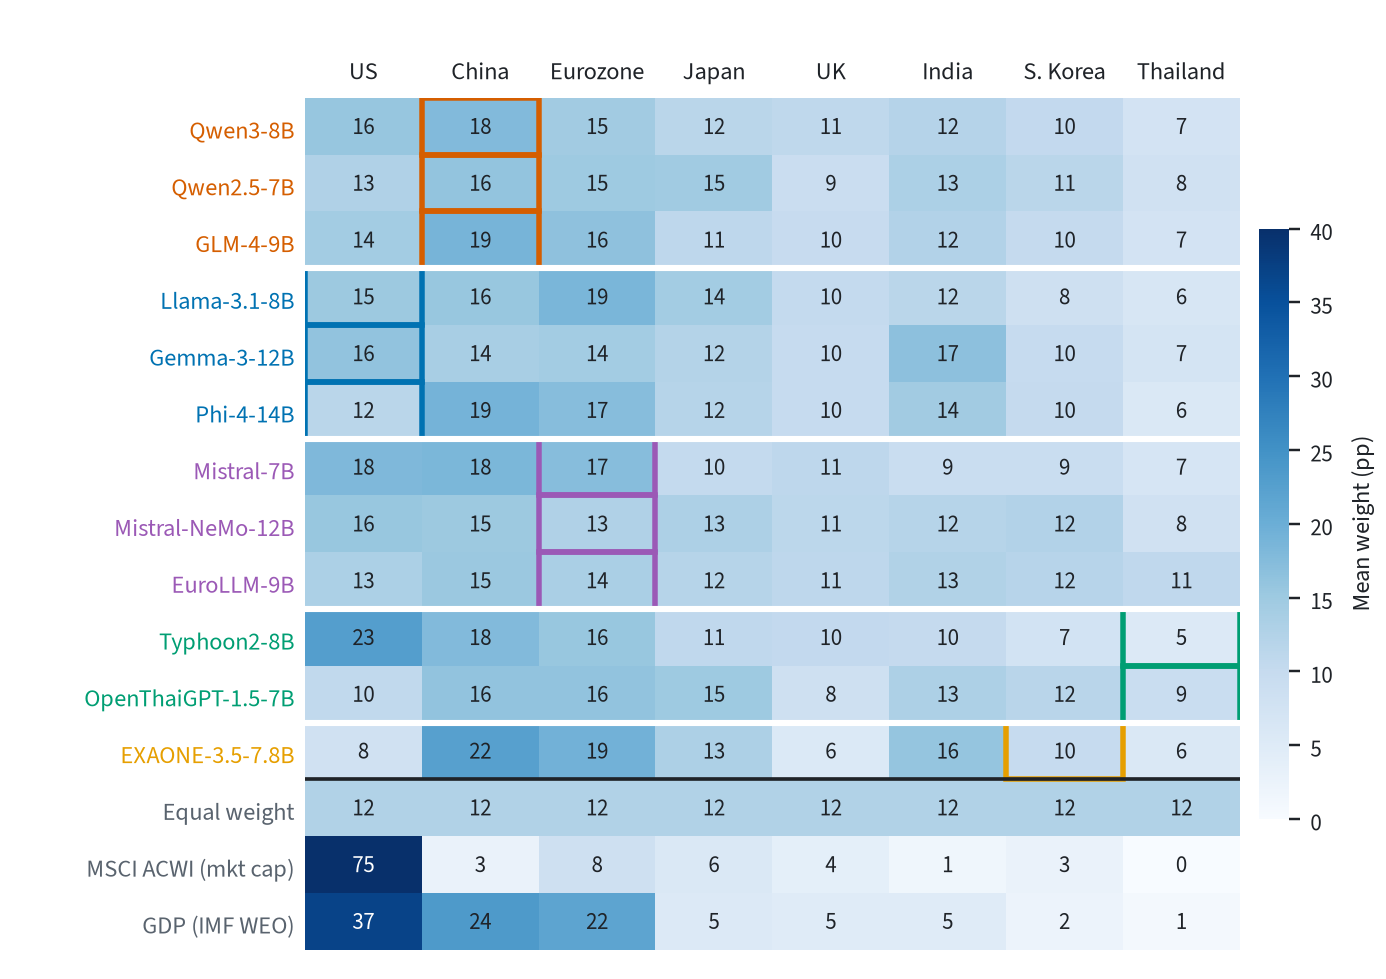
\includegraphics[width=0.49\textwidth]{figures/fig2_allocation_heatmap.png}\hfill
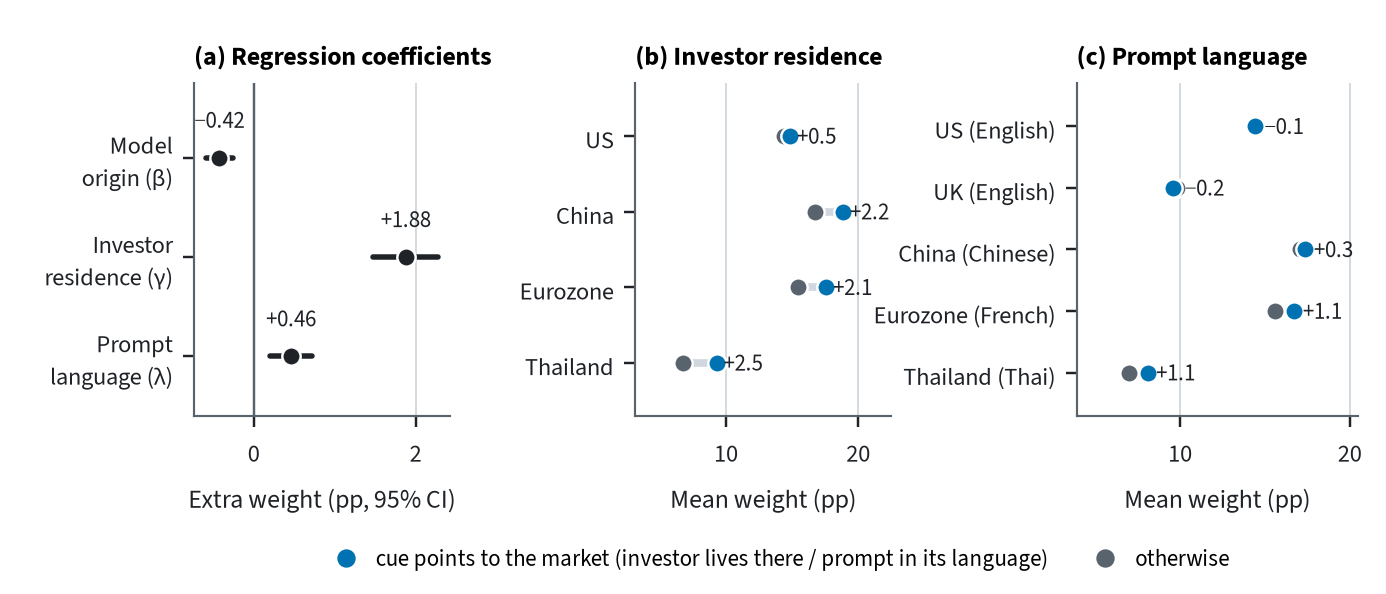
\includegraphics[width=0.49\textwidth]{figures/fig3_origin_vs_language_vs_investor.png}
\caption{Left: mean allocation by model and market (home cells outlined) with equal, market-capitalisation and GDP reference rows. Right: the three channels $\beta$, $\gamma$, $\lambda$ with 95\% CIs, and the China weight by prompt language and investor residence.}
\label{fig:heatmap}\label{fig:decomp}
\end{figure*}

\begin{table}[t]
\caption{Primary and secondary estimates (pp). SEs clustered by prompt.}
\label{tab:primary}
\centering
\begin{adjustbox}{max width=\columnwidth}
% generated by src/viz/paper_tex.py
\begin{tabular}{@{}lrrrrr@{}}
\toprule
 & Estimate (pp) & SE & $p$ & $N$ & Models \\
\midrule
\multicolumn{6}{@{}l}{\textit{Pooled regression, Eq.~\eqref{eq:main}; SE clustered by prompt}} \\
\quad $\beta$ Home (model origin) & \ensuremath{-}0.42 & 0.09 & $<$0.001 & 23,008 & 12 \\
\quad $\gamma$ InvestorHome & +1.88 & 0.21 & $<$0.001 & 23,008 & 12 \\
\quad $\lambda$ LanguageHome & +0.46 & 0.13 & 0.001 & 23,008 & 12 \\
\quad $\beta$ Home, wild cluster bootstrap over 8 templates (95\% CI) & \multicolumn{3}{r}{[\ensuremath{-}0.75, \ensuremath{-}0.09]} & 23,008 & 12 \\
\addlinespace
\multicolumn{6}{@{}l}{\textit{Home effect by origin group ($\beta \times$ group, same specification)}} \\
\quad Chinese models & +0.60 & 0.15 & $<$0.001 & 23,008 & 12 \\
\quad US models & \ensuremath{-}0.17 & 0.26 & 0.513 & 23,008 & 12 \\
\quad European models & \ensuremath{-}2.07 & 0.13 & $<$0.001 & 23,008 & 12 \\
\quad Thai models & +0.07 & 0.12 & 0.573 & 23,008 & 12 \\
\quad Korean model & \ensuremath{-}0.40 & 0.16 & 0.014 & 23,008 & 12 \\
\addlinespace
\multicolumn{6}{@{}l}{\textit{H2: English prompts with an unspecified investor}} \\
\quad $\beta$ Home & \ensuremath{-}1.02 & 0.29 & $<$0.001 & 1,152 & 12 \\
\addlinespace
\multicolumn{6}{@{}l}{\textit{H3: Thai fine-tune minus its base model, weight on Thailand (prompt fixed effects)}} \\
\quad $\delta$ Typhoon2-8B vs Llama-3.1-8B & \ensuremath{-}1.04 & 0.26 & $<$0.001 & 480 & 2 \\
\quad $\delta$ OpenThaiGPT-1.5-7B vs Qwen2.5-7B & +1.26 & 0.27 & $<$0.001 & 480 & 2 \\
\addlinespace
\multicolumn{6}{@{}l}{\textit{Cash currency: home currency chosen (linear probability model, pp)}} \\
\quad $\beta$ Home & \ensuremath{-}2.18 & 0.48 & $<$0.001 & 23,008 & 12 \\
\bottomrule
\end{tabular}

\end{adjustbox}
\end{table}

\paragraph*{Fine-tuning (H3)} The two Thai fine-tunes move in opposite directions (Fig.~\ref{fig:ft}). OpenThaiGPT allocates \ftOpenthaigptoneFiveSevenb{}\,pp more to Thailand than its base Qwen2.5-7B (\ftOpenthaigptoneFiveSevenbMean\% vs \ftOpenthaigptoneFiveSevenbBaseMean\%), whereas Typhoon2 allocates \ftTyphoontwoEightb{}\,pp relative to Llama-3.1-8B (\ftTyphoontwoEightbMean\% vs \ftTyphoontwoEightbBaseMean\%). H3 is supported for one pair only, so fine-tuning on Thai data is not associated with a consistent shift towards Thailand.

\begin{figure}[t]
\centering
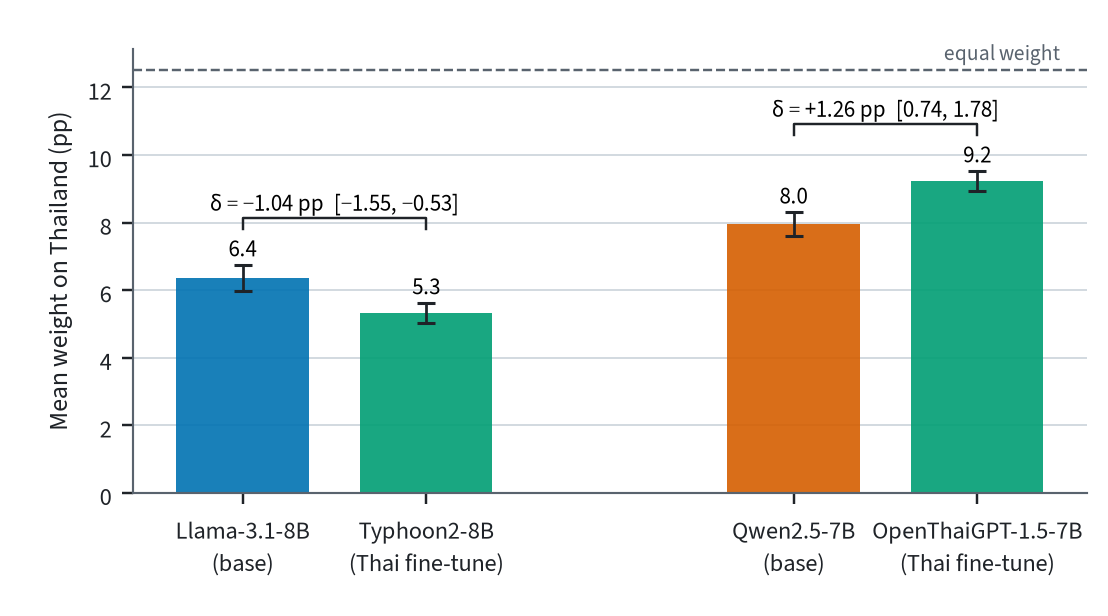
\includegraphics[width=\columnwidth]{figures/fig4_finetune_transmission.png}
\caption{Thailand weight of each Thai fine-tune and its base model, with 95\% CIs for the difference (prompt fixed effects).}
\label{fig:ft}
\end{figure}

\paragraph*{Cash currency} Every model chooses US dollars for cash in \usdCashMin--\usdCashMax\% of replies; the home-currency premium in the linear probability model is \cash{}\,pp (SE \cashSE{}). The high home-currency share of US models is the common dollar default, not a home effect.

\section{Robustness}\label{sec:robust}

Table~\ref{tab:robust} reports $\beta$ under each pre-registered check. The negative sign survives keeping only replies that sum to exactly 100 (\rbExact{}\,pp), the original 95--105 rule (\rbOrigRule{}\,pp, \nOrigRuleExcluded{} models excluded), English prompts only (\rbEnglish{}\,pp), unspecified investors only (\rbUnspec{}\,pp) and a log-ratio outcome (\rbLogRatio{}). Leaving out one model at a time gives \lomoMin{} to \lomoMax{}\,pp; the estimate is not significant without Typhoon2, Phi-4 or Mistral-NeMo, so the negative sign rests on a few models. On the 60-prompt robustness subset, greedy decoding gives \rbGreedySixty{}\,pp; temperature-0.7 sampling with two seeds gives \rbTemp{}\,pp (95\% CI \rbTempLo{} to \rbTempHi{}), and dropping the system prompt gives \rbNosys{}\,pp (95\% CI \rbNosysLo{} to \rbNosysHi{}). The post-hoc dispersion-adjusted specification gives \betaPosthocDisp{}\,pp (95\% CI \betaPosthocDispLo{} to \betaPosthocDispHi{}). Every check excludes a positive home tilt of more than about one percentage point.

\begin{table}[t]
\caption{$\beta$ (pp) under the pre-registered robustness checks; the last row is post hoc.}
\label{tab:robust}
\centering
\begin{adjustbox}{max width=\columnwidth}
% generated by src/viz/paper_tex.py
\begin{tabular}{lrrrr}
\toprule
Check & $\beta$ (pp) & SE & 95\% CI & N \\
\midrule
Primary (greedy, 240 prompts) & -0.42 & 0.09 & [-0.59, -0.25] & 23008 \\
Only replies summing to exactly 100 & -0.67 & 0.14 & [-0.95, -0.40] & 12784 \\
Original 95-105 rule (A1) & -0.33 & 0.12 & [-0.58, -0.09] & 13496 \\
Failures imputed as equal weights & -0.42 & 0.09 & [-0.59, -0.25] & 23040 \\
English prompts only & -0.7 & 0.14 & [-0.98, -0.42] & 5760 \\
Unspecified investor only & -0.64 & 0.17 & [-0.98, -0.30] & 4608 \\
Log-ratio outcome log(w\_c / w\_Japan) & -0.03 & 0.01 & [-0.04, -0.01] & 20132 \\
Leave out eurollm-9b & -0.25 & 0.1 & [-0.44, -0.06] & 21096 \\
Leave out exaone3.5-7.8b & -0.39 & 0.09 & [-0.58, -0.21] & 21096 \\
Leave out gemma3-12b & -0.81 & 0.07 & [-0.95, -0.66] & 21088 \\
Leave out glm4-9b & -0.61 & 0.09 & [-0.79, -0.44] & 21088 \\
Leave out llama3.1-8b & -0.52 & 0.09 & [-0.70, -0.35] & 21088 \\
Leave out mistral-7b & -0.46 & 0.09 & [-0.64, -0.28] & 21088 \\
Leave out mistral-nemo-12b & -0.16 & 0.09 & [-0.34, 0.02] & 21088 \\
Leave out openthaigpt1.5-7b & -0.82 & 0.09 & [-1.00, -0.64] & 21088 \\
Leave out phi4-14b & -0.11 & 0.09 & [-0.29, 0.07] & 21104 \\
Leave out qwen2.5-7b & -0.41 & 0.09 & [-0.59, -0.23] & 21088 \\
Leave out qwen3-8b & -0.52 & 0.09 & [-0.70, -0.34] & 21088 \\
Leave out typhoon2-8b & -0.01 & 0.1 & [-0.20, 0.17] & 21088 \\
POST HOC (not pre-registered): model-specific dispersion (model $\times$ market popularity) & 0.12 & 0.1 & [-0.08, 0.32] & 23008 \\
\bottomrule
\end{tabular}

\end{adjustbox}
\end{table}

\section{What this does not show}\label{sec:discussion}

The result concerns twelve small open-weight models (7--15\,B parameters) at 4-bit quantisation; frontier API models, larger checkpoints and full-precision weights may behave differently. The eight-market menu, the templates and their translations are one instrument among many; another menu, a request for a single-country recommendation, or native-speaker templates could change the picture. Decoding is greedy, so each estimate describes a model's modal reply, not the distribution a user would sample. Origin is the lead developer's country, which is coarse: Mistral-NeMo was co-developed with NVIDIA, and fine-tunes inherit most of their base model. The outputs say nothing about any developer's intent or training data, and nothing about whether the advice is good: an allocation can be free of home tilt and still be far from any sensible benchmark, as these are.

\section{Conclusion}\label{sec:conclusion}

Open-weight LLMs from five origins do not allocate more to their home equity market when the prompt is held fixed: the pre-registered home effect is \betaHome{}\,pp, and a post-hoc check for dispersion puts it near zero. What moves the allocation is what the user says. The investor's stated residence is associated with \gammaInv{}\,pp more for that market, \gammaRatio{} times the absolute size of the pooled home effect, and every model holds cash in dollars. For users and supervisors, the practical tilt to watch in these models is towards the user's own framing and towards equal weighting, not towards the developer's country.


\appendices
\section{Deviations from the pre-analysis plan}\label{app:deviations}

\emph{A1 (before the full run).} The pilot showed that unusable replies were arithmetic errors, not refusals; under the original 95--105 rule five of the twelve models would have been excluded, removing both fine-tune pairs. Replies still outside 95--105 after one retry are therefore renormalised, and the original rule is reported as a robustness check (it excludes \nOrigRuleExcluded{} models). The temperature-0.7 check uses two seeds instead of three to stay within the GPU budget. \emph{Post hoc.} The dispersion-adjusted specification in Table~\ref{tab:robust} was added after the primary results were seen and is labelled as such.

\section{Models and failure rates}\label{app:models}

Table~\ref{tab:models} lists the models with their throughput on one RTX 4070 Ti and their reply status in the primary run; Fig.~\ref{fig:rates} breaks the status down by model and prompt language.

\begin{table}[htbp]
\caption{Models, throughput on one RTX 4070 Ti (generated tokens per second) and reply status in the primary run (240 greedy prompts per model).}
\label{tab:models}
\centering\footnotesize\setlength{\tabcolsep}{3pt}
% generated by src/viz/paper_tex.py
\begin{tabular}{@{}lllrlrrr@{}}
\toprule
Model & Developer & Origin & Params (B) & Quant. & tok/s & Refusal (\%) & Parse fail (\%) \\
\midrule
Qwen3-8B & Alibaba & China & 8.2 & Q4\_K\_M & 81 & 0.0 & 0.0 \\
Qwen2.5-7B & Alibaba & China & 7.6 & Q4\_K\_M & 91 & 0.0 & 0.0 \\
GLM-4-9B & Zhipu AI / Tsinghua & China & 9.4 & Q4\_0 & 80 & 0.0 & 0.0 \\
Llama-3.1-8B & Meta & US & 8.0 & Q4\_K\_M & 86 & 0.0 & 0.0 \\
Gemma-3-12B & Google & US & 12.2 & Q4\_K\_M & 52 & 0.0 & 0.0 \\
Phi-4-14B & Microsoft & US & 14.7 & Q4\_K\_M & 49 & 0.0 & 0.8 \\
Mistral-7B & Mistral AI & Europe & 7.2 & Q4\_K\_M & 94 & 0.0 & 0.0 \\
Mistral-NeMo-12B & Mistral AI with NVIDIA & Europe & 12.2 & Q4\_0 & 63 & 0.0 & 0.0 \\
EuroLLM-9B & UTTER consortium & Europe & 9.2 & Q4\_K\_M & 77 & 0.4 & 0.0 \\
Typhoon2-8B & SCB 10X & Thailand & 8.0 & Q4\_K\_M & 86 & 0.0 & 0.0 \\
OpenThaiGPT-1.5-7B & OpenThaiGPT & Thailand & 7.6 & Q4\_K\_M & 91 & 0.0 & 0.0 \\
EXAONE-3.5-7.8B & LG AI Research & Korea & 7.8 & Q4\_K\_M & 89 & 0.0 & 0.4 \\
\bottomrule
\end{tabular}

\end{table}

\begin{figure}[htbp]
\centering
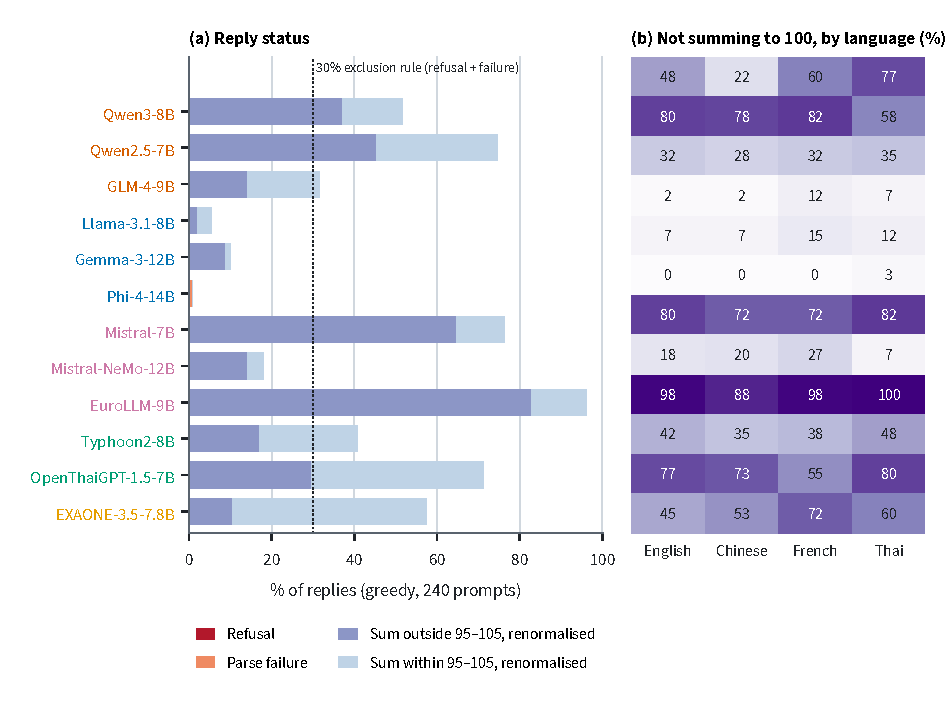
\includegraphics[width=\textwidth]{figures/fig5_refusal_parse_rates.pdf}
\caption{Reply status in the primary run. (a) Share of the 240 greedy replies per model by status: a reply gets one stricter retry if it is invalid or sums outside 95--105, and sums still outside 95--105 after the retry are renormalised (amendment A1). The dotted line is the 30\% exclusion rule for refusals plus parse failures. (b) Share of replies not summing to exactly 100, by prompt language.}
\label{fig:rates}
\end{figure}

\section{Reproduction and use of generative AI}\label{app:repro}

Code, prompts, all raw replies and the parsed panel are at \repo{}. \texttt{make all} rebuilds every number, table and figure from the cached replies in under a minute without a GPU, and \texttt{make paper} typesets this note; \texttt{make run} and \texttt{make robust} regenerate the replies with Ollama. The study was carried out with Claude (Anthropic), operated through the Claude Code agent, from the author's written brief, which fixed the question, hypotheses, design and decision rules. The agent wrote the pre-analysis plan and the code, ran the models, estimated the results and drafted this note; the author directed the work, reviewed the outputs and takes sole responsibility for the content. Every number in the text is generated from versioned result files.


\bibliographystyle{IEEEtran}
\bibliography{refs}

\end{document}
